\chapter{Insertar pdf}

Si se quiere incluir un pdf, se puede utilizar el comando \verb!\includepdf{./pdf/nombre}!, donde ./pdf/ es el directorio donde está guardado el pdf, y "nombre" es el nombre con el que está guardado el pdf.


\includepdf{./pdf/LOGOS}

Por defecto, sólo se inserta la primera página. En caso de pdf con más de una página, se puede escoger qué páginas insertar, o insertarlas todas. Con \verb!\includepdf[pages=2]{./pdf/nombre}! se inserta la segunda página.


\includepdf[pages=2]{./pdf/LOGOS}

Y con \verb!\includepdf[pages=-]{./pdf/nombre}! se insertan todas las páginas.


\includepdf[pages=-]{./pdf/LOGOS}

En caso de pdf que estan configurados en horizontal, por defecto se insertan en orientación horizontal en la página en vertical.

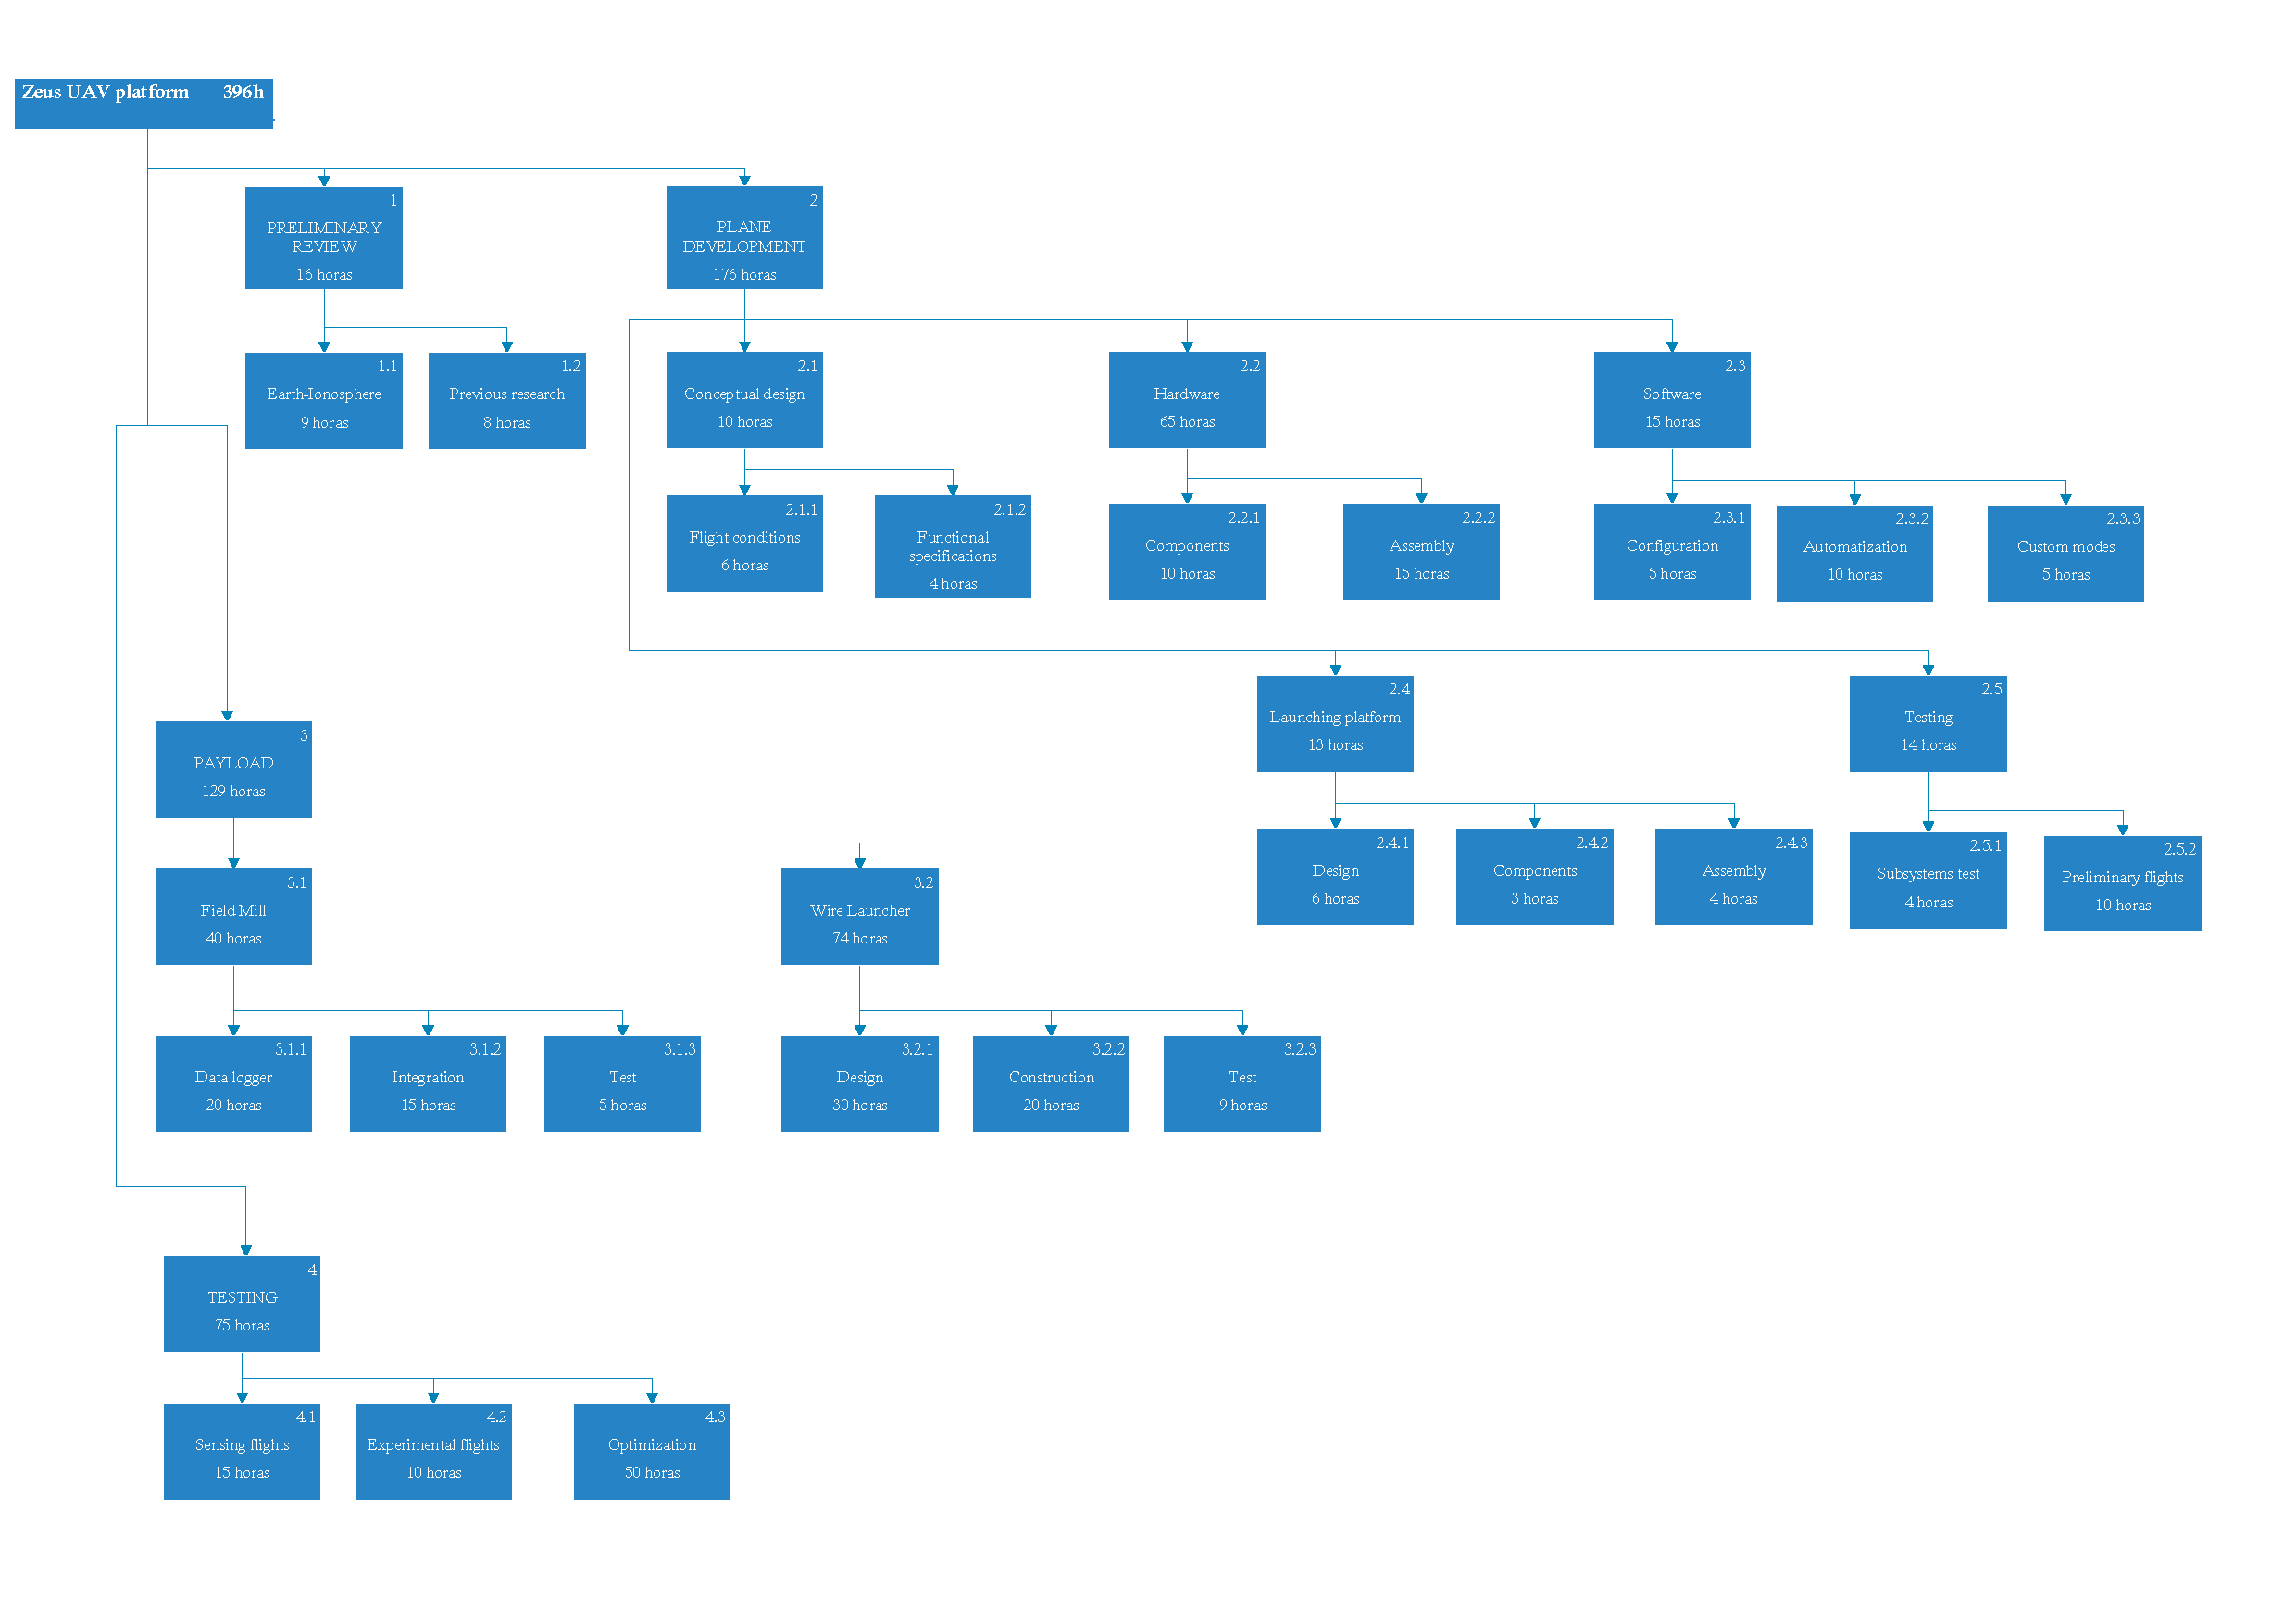
\includepdf{./pdf/WBS}

Si se quiere que la página también esté en horizontal, hay que utilizar \verb!\includepdf[landscape=true]{./pdf/nombre}!

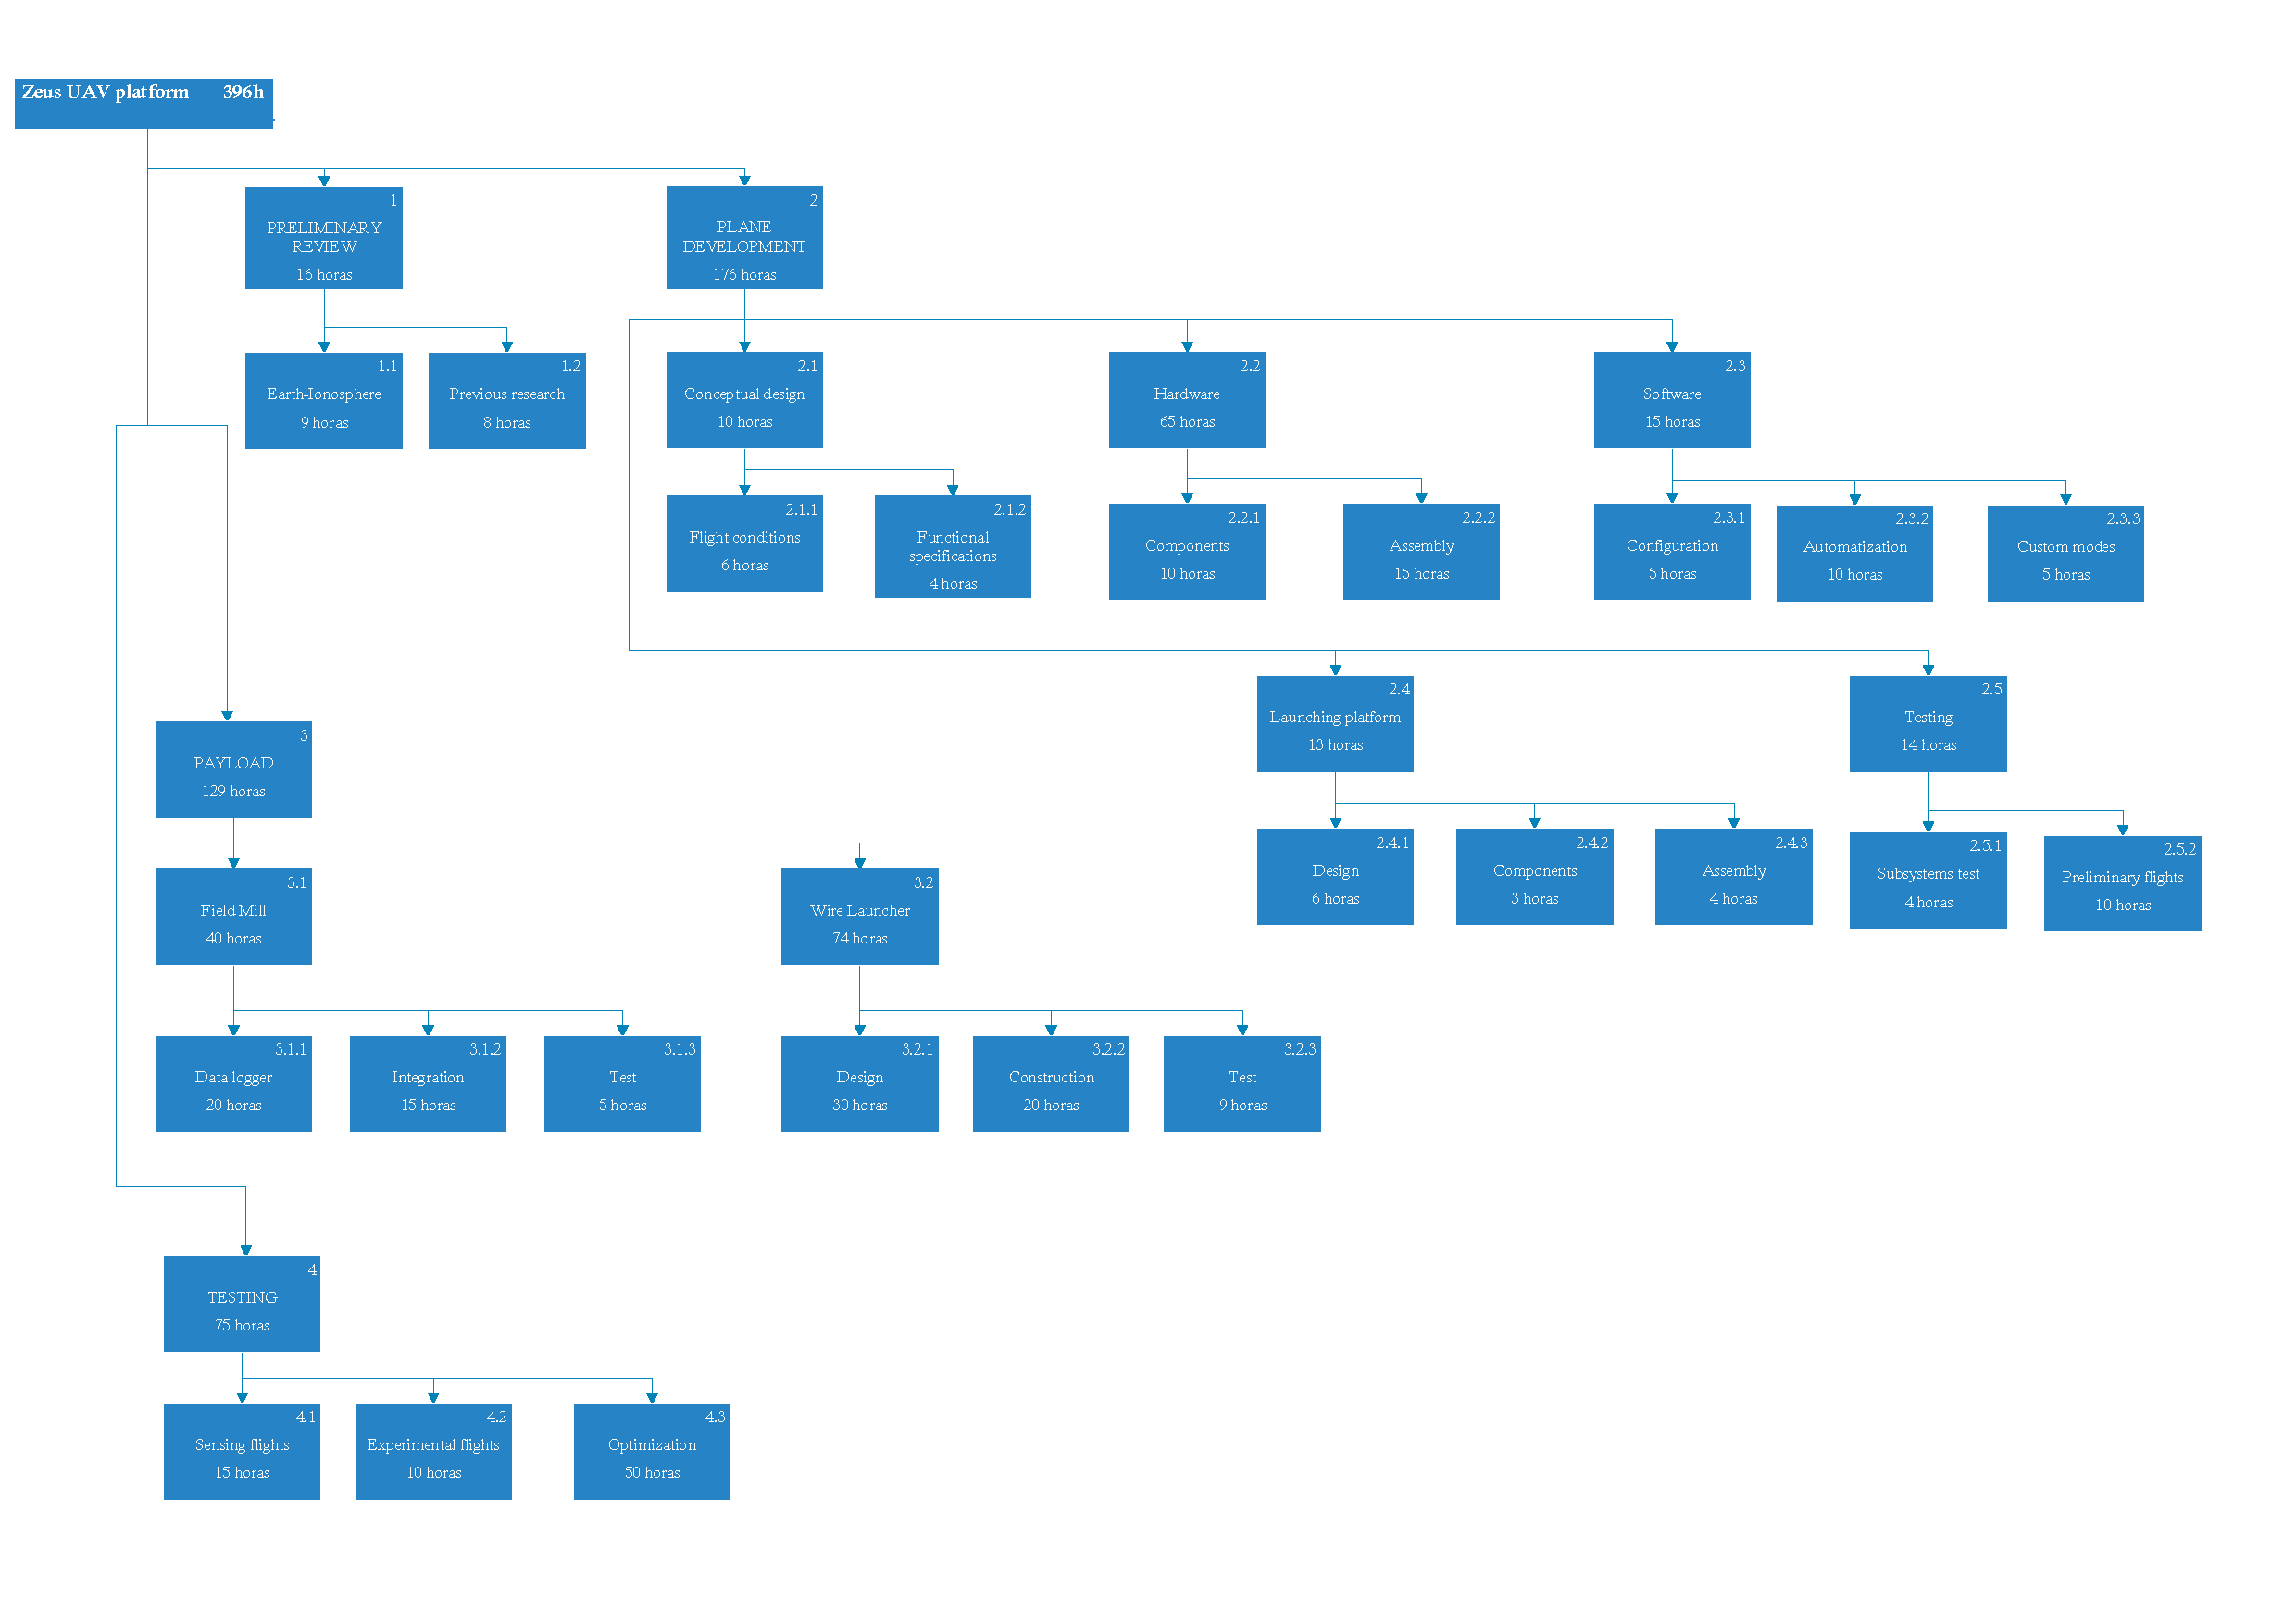
\includepdf[landscape=true]{./pdf/WBS}

Y para el número de páginas se aplica lo explicado anteriormente. Utilizando el comando \verb!\includepdf[landscape=true,pages=-]{./pdf/nombre}!, se insertan todas las páginas del pdf con la orientación de las páginas en horizontal

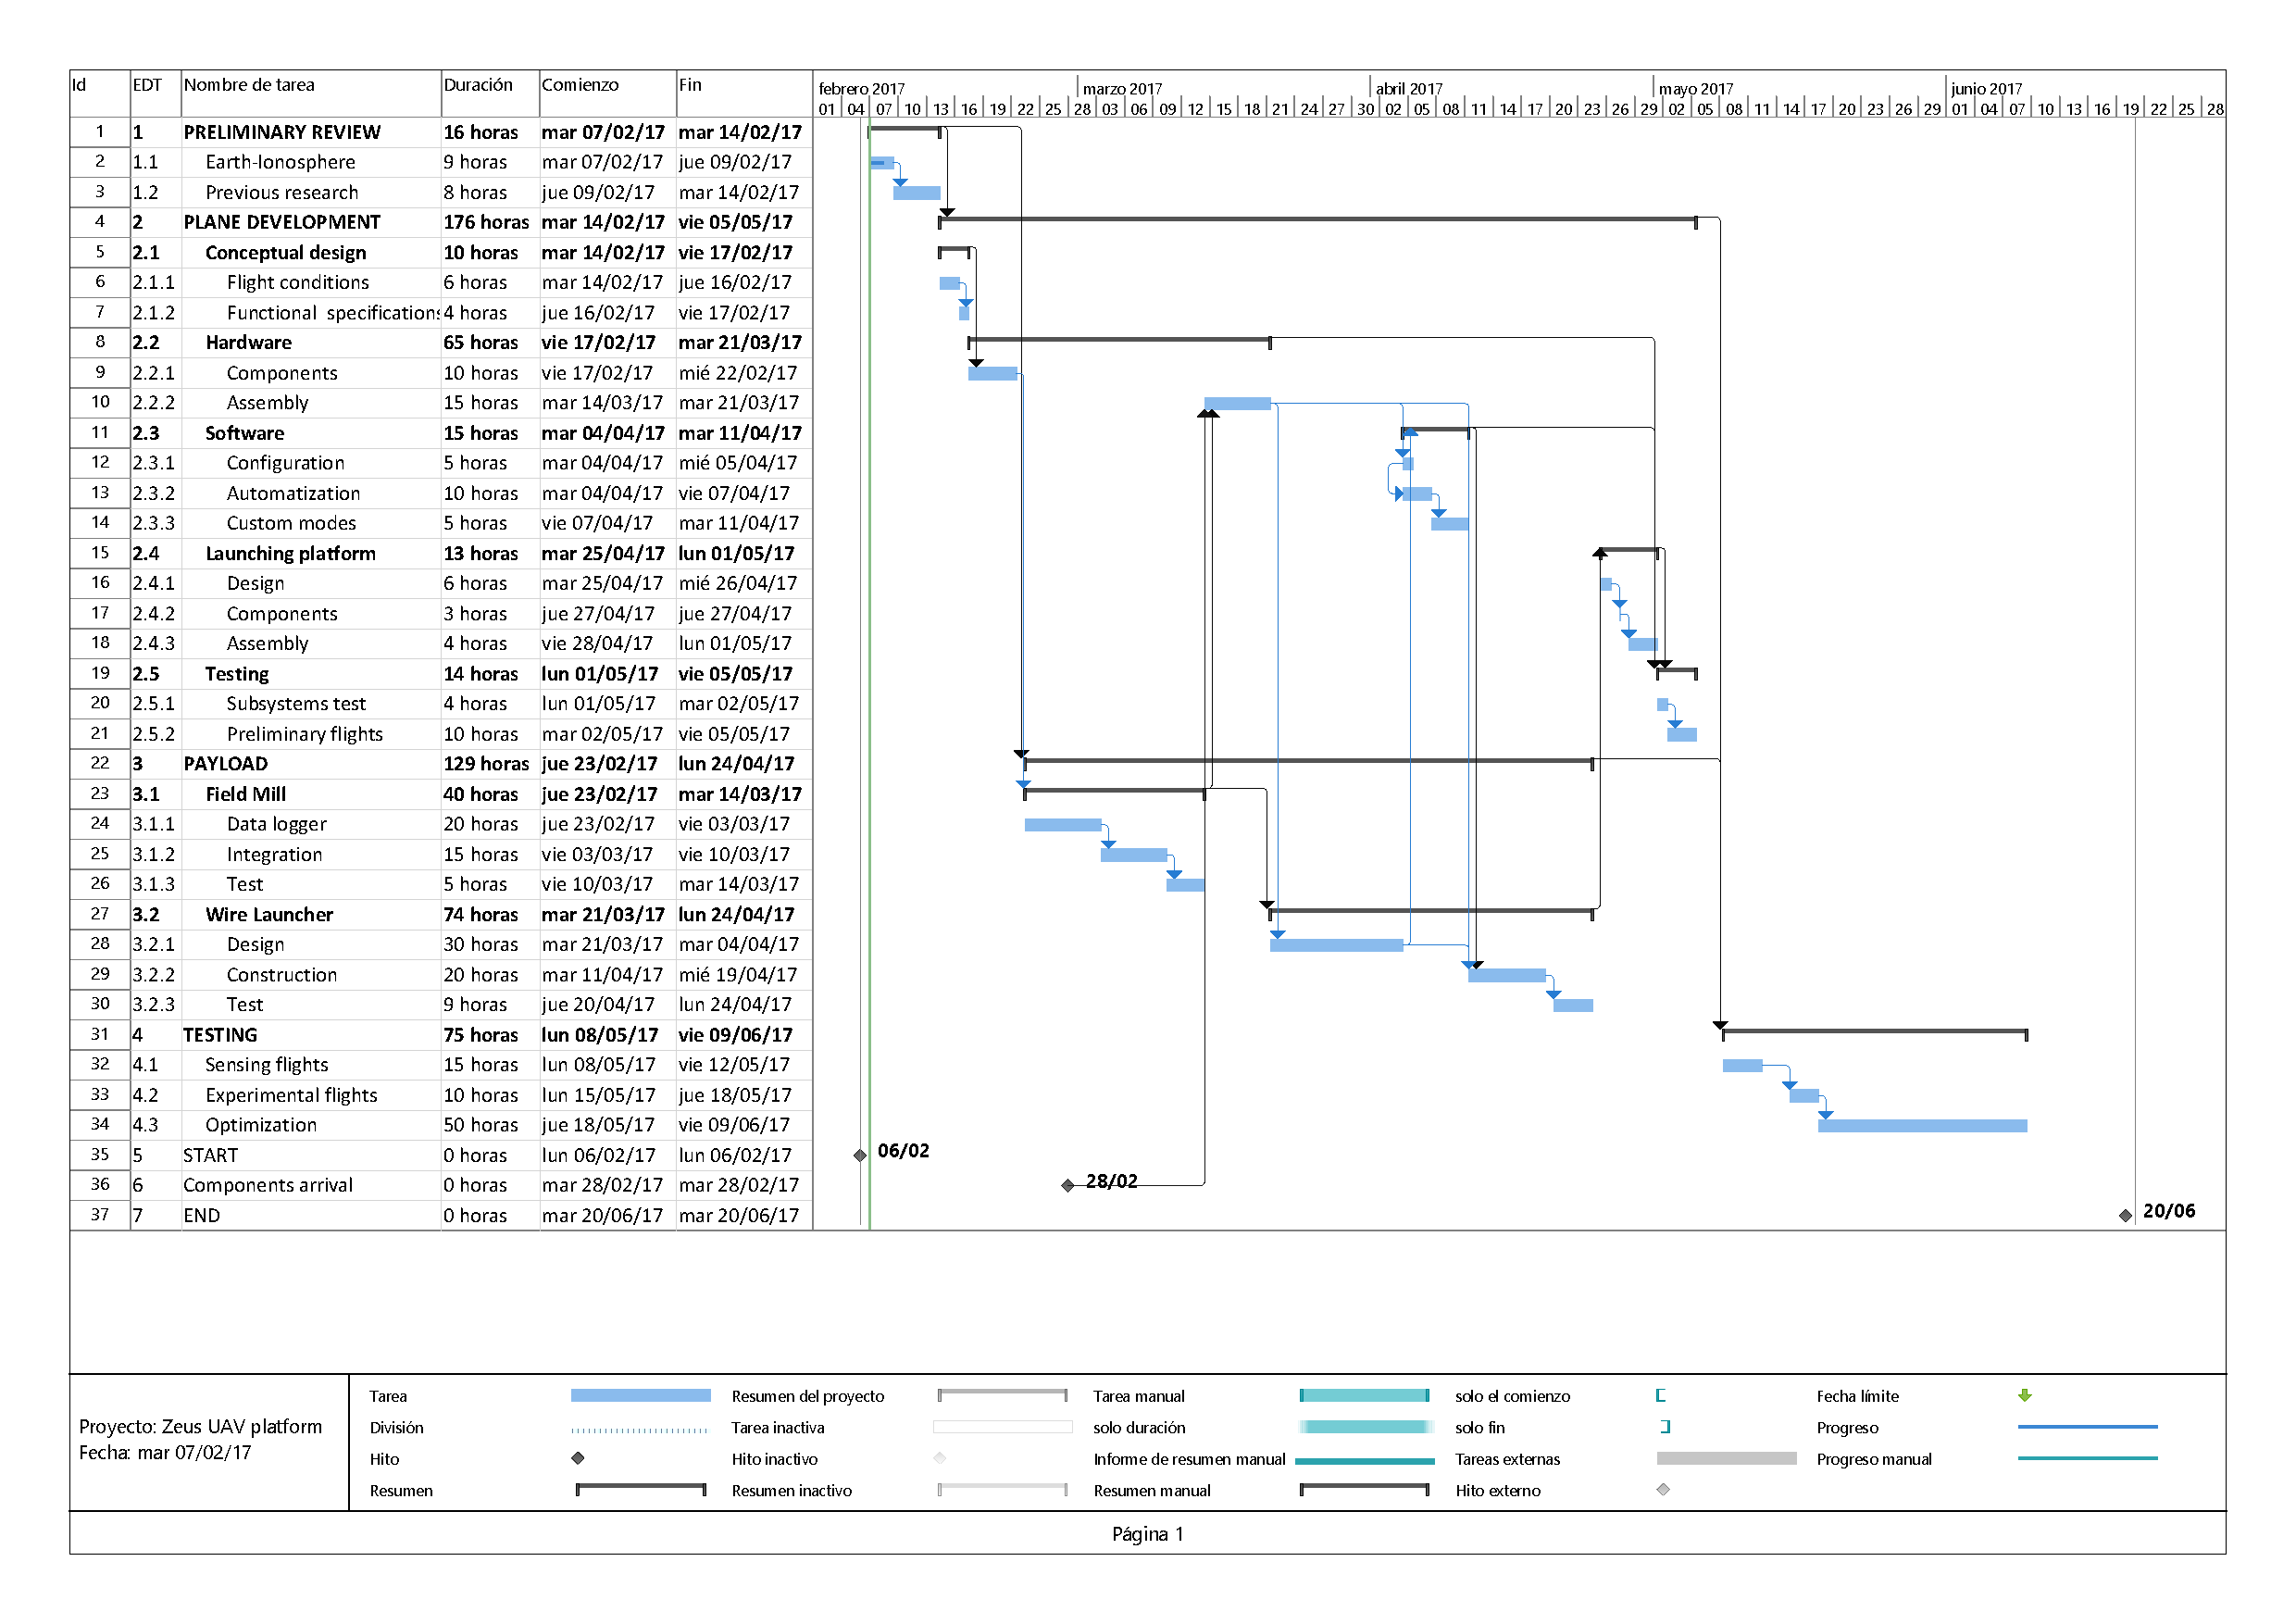
\includepdf[landscape=true,pages=-]{./pdf/GANTT}